%\documentclass[nynorsk]{ifimaster}  %% ... or USenglish or norsk or nynorsk
\documentclass[oneside, nynorsk]{book}
\usepackage[utf8]{inputenc}           %% ... or latin1 or applemac
\usepackage[T1]{fontenc,url}
\urlstyle{sf}
\usepackage{babel,textcomp,csquotes,ifimasterforside,varioref,graphicx}
\usepackage[backend=biber,style=numeric-comp]{biblatex}

\usepackage{amsfonts}
\usepackage{amsmath}
\usepackage{mathtools}
\usepackage{empheq}
\usepackage{systeme} % likninger

\usepackage{graphicx}
\usepackage{caption}
\usepackage{subcaption}
\usepackage{float}

\setlength\parindent{0pt}
\setlength\parskip{\medskipamount}

% 2c. For norske tegn
\usepackage[T1]{fontenc}
\DeclareUnicodeCharacter{0177}{\^y}
%\DeclareUnicodeCharacter{0302}{\^x}

\renewcommand{\thesubsection}{\alph{subsection})}
\newcommand*\widefbox[1]{\fbox{\hspace{2em}#1\hspace{2em}}}

%\addbibresource{kjelder.bib}

\title{Prosjekt 3}        %% ... or whatever
\subtitle{FYS-STK4155 --- Applied data analysis and machine learning}         %% ... if any
\author{Espen Næss}                      %% ... or whoever

\bibliography{mybib}                  %% ... or whatever

\begin{document}
\let\cleardoublepage\clearpage
\ififorside{}
\let\cleardoublepage\clearpage
\chapter*{Abstrakt}                   %% ... or Sammendrag or Samandrag
Målet med prosjektet er å undersøkja diverse maskinlæringsalgoritmar for å klassifisera om ein pasient har eit epileptisk anfall eller ikkje
basert på målingar av elektrisk aktivitet i hjernebarken (EEG-data).
Prosjektet oppnådde gode resultat. Med berre eit sekund med måledata vart det mogleg med
ei klassifiseringsgrannsemd på $0.971$ for det sjølvimplementerte nevrale nettet frå prosjekt 2 om det vart gjort ei god eigenskapsuttrekking på førehand. Liknande resultat vart òg oppnådde med scikit learn og keras sine implementeringar.

RNN/LSTMar kravde inga eigenskapsuttrekking og kom opp i ei grannsemd på $0.963$ på sitt beste,
men det er stort sannsyn for at parameterrommet vart dårleg undersøkt då det vart særs tidskrevjande å trena dei ulike LSTM-modellane.
Det beste resultatet for logistisk regresjon vart $0.965$ i grannsemd med $10^{-2}$ i straffeparameter med ein tilhøyrande l1-norm.
Støttevektormaskiner kom opp i ei grannsemd på $0.97$ med ein polynomiell kernelfunksjon eller ein GRB kernelfunksjon og fekk altså eit resultat særs likt resultat som for dei nevrale nettverka.

Koden for heile prosjektet finst på den følgjande githubadressa: \\
https://github.com/EspenNaess/Prosjekt-3-FYS-STK4155
\tableofcontents{}
%\listoffigures{}
%\listoftables{}
\mainmatter{}
\chapter{Introduksjon}                    %% ... or Forord
Epilepsi ein av dei mest utbreidde nevrologiske sjukdommane i verda - kring 10 prosent av verda si befolkning
vil få eit uprovosert epileptisk anfall utløp av livet sitt \cite{Epil}.
Eit epileptisk anfall er raske og ukontrollerte avfyringar av nerveceller i særskilde område av hjernen.
Kvar nervecelle kan i eit epileptisk anfall avfyra opptil 500 gongar per sekund
i motsetning til vanleg nervecelleaktivitet som ligg ved 80 avfyringar per sekund \cite{Epil2}.

Om desse ukontrollerte avfyringane er avgrensa til særskilde område av hjernen gjev dette milde symptom \cite{Epil3}.
Ein pasient kan til dømes vera ute av stand til å formulera samanhengande setningar om nerveceller ansvarlege for tale vert overbelasta av desse ukontrollerte avfyringane.
Samstundes er det ofte at desse ukontrollerte avfyringane spreier seg til heile hjernen.
Eit slikt anfall vert kalla eit grand mal anfall \cite{Epil3}.
Dette er den mest alvorlege typen anfall og fører til at pasienten fell om, mistar medvitet, ristar ukontrollert og frodar.
Varer anfallet meir enn fem minutt kan pasienten i verste fall døy.

Målet med dette prosjektet er å klassifisera desse grand mal anfalla hjå pasientar basert på målingar frå eit EEG-måleapparat.
Pasienten får sugekoppar frå EEG-måleapparatet festa på hovudet som måler elektrisk aktivitet i særskilde område av hjernebarken. Desse målingane vert til EEG-signal.
Målet med prosjektet er å klassifisera desse signala ved ulike maskinlæringsmetodar som anten ei måling av eit epileptisk anfall eller ikkje.

Eit automatisk system som detekterer anfall har vore eit heitt tema innanføre forskinga på nytt medisinsk utstyr.
Ei manuell tolking av EEG-signal er ikkje ei triviell oppgåve og krev godt trente nevrofysiologar \cite{Epil4}.
Det er òg ei einsformig og tidkrevjande oppgåve å gjera manuelt samstundes som denne metoden er særs disponert for menneskelege feil.
Bruk av maskinlæring for anfallsdetektering vil òg ideelt opna opp for at deteksjon av eit anfall kan henda tidlegare enn ved bruk av dei manuelle metodane, då
maskinlæringsteknikkane ideelt kan sjå mønstera ein større samanheng.
Dette er særs viktig om anfalla er så alvorlege at pasienten kan mista livet av dei.
\chapter{Teori og metodar}                  %% ... or Bakgrunn
I denne rapporten vil teori knytt til logistisk regresjon og MLPar nyttast.
Denne teorien er greidd godt ut for i rapport 2, så det vert referert til
rapport 2 for teorien bak logistisk regresjon og MLPar \cite{Naess}.
\section{Oppsett av data}
Datamengda utgjer 500 EEG-målingar frå 500 personar. 100 av dei hadde eit epileptisk anfall under målinga, medan 400
hadde inkje anfall. Kvar EEG-måling utgjer ei 23.6 sekund langt signal som er sampla med ein samplingsrate på 173.6 Hz.
Dette gjev 4097 datapunkt i det digitale signalet. Vidare vert signalet delt inn i 23 oppdelingar.
Dette er så ei oppdeling femner kring ei eitt sekunds måling.

Totalt vert det altså $500*23=11500$ signal som kan verta nytta til trening/testing.
Datamengda utgjer ei matrise der kvar rad utgjer eit sampel av eitt sekund langt signal av ei EEG måling.
I dette høvet er det 178 målepunkt for eitt sekund som utgjer kvar eigenskapsvektor.
Vidare er $y$-verdiane særskilde taggar for dataen - eit epileptisk anfall eller ikkje.

Koden for innlastinga av datamengda ligg i «LastData.py» med einingstestar for at datamengda fungerer som ho skal.
\newpage
\section*{Eigenskapsuttrekking av datamengda}
Datamengda vil utgjera kring 11500 signal med 178 datapunkt.
MLPar har ikkje minne over sekvensiell data i motsetnad til andre nevrale nettverk som RNN,
så å gjeva signala til ein MLP utan noka form for preprossessering vil vera fåfengt. Det same gjeld òg for andre metodar som logistisk regresjon og
støttevektormaskiner.
Skal desse metodane klassifisera desse signala vert det difor naudsynt med ei eigenskapsuttrekking av signala.
I dette høvet vart gjennomsnitt, standardavvik, kurtose, skeivskap samt verdiar for min/max valde som eigenskapar ut i frå Fig. ~\ref{Episignal}.

\begin{figure*}[h!]
  \begin{subfigure}{\textwidth}
        \centering
        \centerline{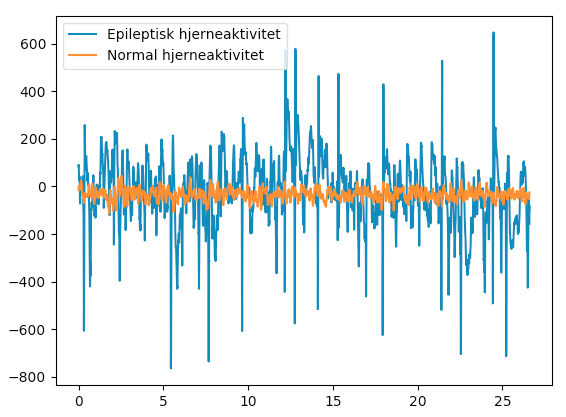
\includegraphics[width=0.8\linewidth]{Signalsamanlikn}}
        \caption{Døme på eit EEG-signal med normal hjerneaktivitet og eit med epileptisk hjerneaktivitet.
        Det er tydeleg at det vert større utslagsverdiar for eit epileptisk signal. Kurtose samt. verdiar for min/max er såleis gode eigenskapar.
        Det er forventa ein større varians samt. gjennomsnitt i eit epileptisk signal
        enn i eit signal med vanleg aktivitet, så desse vert òg viktige eigenskapar.
        Merk at sjølv om det her kan sjå trivielt ut å klassifisera dei to signala ved øyemål, er det som nemnt i introduksjonen særs vanskeleg og krev godt trente nevrofysiologar.
        Totalt vart følgjande eigenskapar valde for å skilja mellom signala; gjennomsnitt, standardavvik, kurtose, skeivskap samt verdiar for min/max.}
        \label{Episignal}
    \end{subfigure}
\end{figure*}

Det er venta at dei valde eigenskapane vil skildra mykje av den same informasjonen, så det vert gjort ei redusering av eigenskapar basert på prinsipalkomponentanalyse (PCA).
\newpage
\section{Eigenskapsuttrekking ved PCA}
Om to eigenskapar er like anten i verdi eller korrelasjon så er dei overflødige. Ein kan då gjera ein prinsipalkomponentanalyse for å redusera talet på
eigenskapar. % Dette kan hjelpa med overfitting då metoden reduserer variansen til modellen som vert tydeleg frå utrekningane i denne seksjonen.
Generelt kan ei eigenskapsuttrekking skildrast som ei lineæravbildning. Ein ønskjer å finna ei optimal avbildning frå alle eigenskapane
til ei meir avgrensa mengde av eigenskapar.
Gjeve eit eigenskapsrom X skal ein altså finna ei avbildning $x_i \in X$ sånn at:
\[y=f(x_i)\]
Som gjev redusert dimensjon på y vektoren i høve til $x_i$.
Målet med PCA er å finna ei lineæravbildning
som gjev ukorrelerte eigenskapar samstundes som rekonstruksjonsfeilen mellom original og transformert data vert minimal.
Dette kan verta oppnått ved ei lineæravbilding $y=A^Tx_i$. % der $y$ er ukorrelerte.

Kvar og ein komponent i vektoren $y$ kan ein tenkja på som resultatet av ein projeksjon av x på ein av radvektorane $w_i$ i $A^T$, gjeve at
A er ei matrise med kolonnar gjevne som $A=[w_1 \quad .. \quad w_n]$.
Til dømes vil $y_1=w_1^Tx$ og om $y_1$ vert normalisert så får ein lengda av den projekterte vektoren x på $w$:
\[|proj_{Span(\{w_1\})}x|=\frac{w_1^Tx}{w_1 \cdot w_1}\]
Altså vil komponentane i resultatet av lineæravbildninga for PCA i røynda vera resultatet av projekteringar
på radvektorane i transformmatrisa, bunde av at resultatvektoren $y$ vert normalisert.

Eitt av måla med transformasjonen var at rekonstruksjonsfeilen mellom original og transformert data vert minimal.
Målet er altså å minimisera MSE mellom $x_i$ og $y_i$. Uttrykket for MSE kan gjerast enklare ved at:
\begin{align*}
||x_i-y_i||^2&=||x_i-(w\cdot x_i)w||^2 \\
&= (x_i-(w\cdot x_i)w)\cdot (x_i-(w\cdot x_i)w) \\
&= x_i\cdot x_i-x_i \cdot (w\cdot x_i)w-(w\cdot x_i)w\cdot x_i+(w\cdot x_i)w\cdot (w\cdot x_i)w \\
&= ||x_i||^2-2(w\cdot x_i)^2+(w\cdot x_i)^2\cdot w \cdot w \\
&= ||x_i||^2-2(w\cdot x_i)^2+(w\cdot x_i)^2 \\
&= x_i\cdot x_i - (w\cdot x_i)^2
\end{align*}
Ein får altså frå uttrykket ovanføre at
\[||x_i-y_i||^2=||x_i||^2-y_i^2\]
Tek ein MSEen av dette vert det:
\[MSE=\frac{1}{N}\sum_{i=1}^n ||x_i-y_i||^2=\frac{1}{N}\sum_{i=1}^n ||x_i||^2-y_i^2=\frac{1}{N}\left(\sum_{i=1}^n ||x_i||^2 - \sum_{i=1}^n y_i^2\right)\]
Så det å minimisera MSE er det same som å maksimera dette følgjande gjennomsnittet: $\sum_{i=1}^n y_i^2$.
Gjennomsnittet av ei kvadrering er alltid lik ei kvadrering av gjennomsnittet pluss variansen og kjem frå statistikken.
Då har ein at:
\[\sum_{i=1}^n y_i^2=\sum_{i=1}^n (w\cdot x_i)^2=\left(\frac{1}{n}\sum_{i=1}^n x_i \cdot w \right)^2+Var[w\cdot x_i]\]
Men samstundes så vil $\left(\frac{1}{n}\sum_{i=1}^n x_i \cdot w \right)^2$ vera 0, då den projekterte datamengda har 0 i gjennomsnitt som jo
var føresetnaden for alle desse utrekningane. Så MSE vert enkelt og greitt:
\[MSE=\frac{1}{N}\left(\sum_{i=1}^n ||x_i||^2 - Var[w\cdot x_i]\right)\]
Så det å minimisera MSE er ekvivalent med å maksimera $Var[w\cdot x_i]=Var[y_i]$.
Ein ønskjer altså størst varians på mengda av $y$-vektorar som òg gjev meining intuitivt, då større varians gjer at meir informasjon vert skildra.
Variansen for $y$ er (gjeve at x er substrahert med gjennomsnittet)
\[\sigma_w^2=\frac{1}{N}\sum_{i}y_i^2=\frac{1}{N}\sum_{i}(w^Tx_i)^2=w^T(\frac{1}{N}\sum_{i}x_ix_i^T)w=w^TRw\]
Ut frå utrekninga er det tydeleg at R er kovariansmatrisa for datamengda $X$.

Så målet nå er å maksimera denne variansen for å løysa problemet. Tidlegare vart det utleitt at variansen for y er
$\sigma_w^2=w^TRw=J(w)$ som ein ønskjer å maksimera. Løysinga av dette problemet vert kvadratformpensum frå lineæralgebraen,
evt så kan det gjerast med lagrangemultiplikator $J(w)$ som skal maksimerast under føresetnaden om at w er ein normalisert vektor.

Som kjent frå lineæralgebraen vil det å maksimera funksjonar på forma $J(w)=w^TRw$ svara til eigenvektoren w som svarar til den største eigenverdien for matrisa R.
Eigenvektoren til matrisa R som svarar til den største eigenverdien vil altså maksimera $J(w)$. Ein kan koma fram til same resultat med lagrangemultiplikatorar.
Vidare kan det verta vist at dei andre vektorane som maksimerer $J(w)$ òg er eigenvektorar gjevne i stigande rekkjefølgje etter eigenverdi.
Dette kan verta utleitt frå kovariansen definert ovanføre.
Kovariansen mellom to komponentar $y_n$ og $y_m$ er gjeven som:
\[COV=\frac{1}{N}\sum_{i}^Ny_n(i)^Ty_m(i)=\frac{1}{N}\sum_{i}^Nw_n^Tx(i)x(i)^Tw_m=w_n^TRw_m\]
Målet var at $y$-komponentane skal vera ukorrelerte. Kovariansen må altså vera 0 mellom y-komponentane. altså må $w_n^TRw_m=0$ som er ekvivalent med å krevja at
$w_nw_m=0$. Med di maksimum av $J(w)$ er den eigenvektoren som har størst eigenverdi og det òg er kravt at dei andre w-ane er normale til denne eigenvektoren, så følgjer det at
dei andre w-vektorane må vera eigenvektorar som følgje av at eigenvektorar er lineært uavhengige av kvarandre.
Alle desse eigenvektorane er kjende som prinsipalkomponentane i algoritmen.

PCA vert vidare gjort ved den følgjande lineæravbildninga
\[y=A^Tx_i \qquad \text{gjeve at $A=[w_1 \quad .. \quad w_n]$}\]
der w-ane er prinsipalkomponentane utleidde ovanføre.
Som følgje av teorema viste ovanføre så vil $y$ ha ukorrelerte element og så høg varians som mogleg,
samstundes som at eigenskapsreduseringa gjev den beste MSEen sett i høve til originaldatamengda.

Med kovariansmatrisa kan ein redusera talet på variablar. Den totale variansen er gjeven som summen av diagonalen i kovariansmatrisa R.
Skildrar ein komponent på diagonalen ein låg prosentdel av den totale variansen kan denne komponenten verta utelaten.

%Det finst geometriske tolkingar av prinsipalkomponentane. Vektoren med første prinsipalkomponent (eigenvektoren med størst eigenverdi) er ein vektor i scatterplottet som
%går langs den lengste aksen av datapunkta i scatterplottet. Andre prinsipalkomponent står vinkelrett på hin vektoren etc.

\section{Støttevektormaskiner (SVM)}
\begin{figure*}[h!]
    \centering
    \centerline{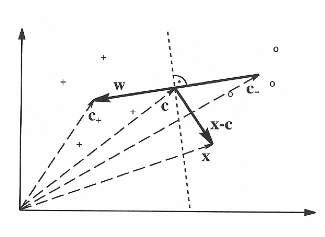
\includegraphics[width=0.6\linewidth]{SVM}}
    \caption{Her er $c_{+}$ og $c_{-}$ forventningsverdiane for kvar si fordeling over features knytte til kvar av dei to klassene som det skal klassifiserast til.
    Det vert definert ei lineær avgjerdsgrense som står vertikalt på vektoren $w=c_{+}-c_{-}$ som svarar til den stripla linja i biletet.
    Her er $x$ eit nytt sampel ein ønskjer å klassifisera. Ut i frå dette viser det seg at ein kan motivera nytta til støttevektormaskiner.}
    \label{SVM}
\end{figure*}
For å klassifisera eit sampel $x$ vil eit vettugt utgangspunkt vera å sjå om den absolutte vinkelen som er utspend av vektoren $x-c$ frå $w$ er mindre enn $\frac{\pi}{2}$ for å sjå kva for ei side av avgjerdsgrensa sampelet x finst på.
Kall denne vinkelen $\alpha$. Då vil $\cos(|\alpha|)>0$ om sampelet er på den eine sida av avgjerdsgrensa og $\cos(|\alpha|)<0$ om sampelet er på den andre sida.
Denne cosinusrelasjonen kan skildrast ved eit indreprodukt gjennom relasjonen om at
\[cos \theta = \frac{w \cdot x}{||w|| ||x||} \qquad \text{der $\theta$ er vinkelen mellom vektorane w,x}\]
Dette svarar til indreproduktet mellom forventningsvektoren $w=c_{+}-c_{-}$ og vektoren frå $w$ til
punktet x ein skal klassifisera. Eit punkt x på avgjerdsgrensa gjeve som ein vektor oppfyller $w\cdot x=0$.
Om avgjerdsgrensa vert skoven ved å leggja til ein bias får ein essensielt avgjerdsgrensa for ei støttevektormaskin:
%Ein går ut frå at avgjerdsgrensa kan verta skriven som
%\[g(x)=w^Tx + b=w_1x_1+..+w_lx_l+b=0\]
%Dette er eit hyperplan i eit l-dimensjonelt eigenskapsrom. Avgjerdsgrensa er som sagt $w^T(x_1-x_2)=0$, med di $w$ er ortogonal til avgjerdsgrensa, som i Fig. ~\ref{Dome}.
%Eit bevis for det er at om to punkt $x_1,x_2$ er på avgjerdsgrensa vil $w^Tx_1 + b=w^Tx_2 + b=0$ som gjev $w^T(x_1-x_2)=0$.
%Ein ønskjer altså ei delelinje:
\[g(x)=w^Tx + b=w_1x_1+..+w_lx_l+b=0\]
Dette er eit hyperplan i eit l-dimensjonelt eigenskapsrom.

$\frac{g(x)}{||w||}$ for eit sampel x er avstanden mellom sampelet x og avgjerdsgrensa.
Dette kan ein sjå på som ein ortogonal projeksjon på eit underrom utspent av vektoren $w$.
\[\frac{g(x)}{||w||}=\frac{w^Tx + b}{w\cdot w}=\frac{w \cdot x + b}{w\cdot w}=\frac{x \cdot w}{w\cdot w}+ \frac{b}{w\cdot w}\]
Vektoren $\frac{x \cdot w}{w\cdot w}w$ ville vore ein prosjeksjon av vektoren x på w, men $\frac{x \cdot w}{w\cdot w}$ åleine gjev berre lengda av denne vektoren.
 \begin{figure*}[h!]
     \centering
     \centerline{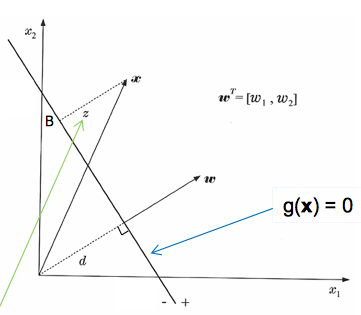
\includegraphics[width=0.6\linewidth]{SVMmath}}
     \caption{Målet er å finna avstanden frå eit sampel x til avgjerdsgrensa. Grafisk gjev det meining å prosjektera på w og henta ut lengda av denne projekterte vektoren, då w vil alltid vera ortogonal til avgjerdsgrensa $g(x)=0$.}
     \label{SVMmath}
 \end{figure*}

%\[w^Tx + b>1\]
%\[w^Tx + b<1\]
%Dette gjev to nye grensevektorar som vert kalla støttevektorar, sjå Fig ~\ref{SVMbilete}.
%\[w^Tx + b=1 \qquad w^Tx + b=-1\]

Målet vidare er å finna ein vektor $w$ av vekter og ein bias $b$ som gjev den maksimale marginen, sjå Fig ~\ref{SVMbilete}.
Det vert det same som å minimisera nemnaren til marginen, altså å minimisera den følgjande funksjonen:
\[J(w)=\frac{1}{2}||w||^2 \qquad \text{gjeve føresetnaden $y_i(\frac{g(x_i)}{||w||})\geq \frac{1}{||w||}$}, \forall i\]
$\frac{1}{2}$ framføre uttrykket gjev enklare utrekningar og er der difor av konvensjon, elles ingen annan grunn til at han er der.
$y_i$ er klasselabelen for sampel $x_i$, anten -1 eller 1. Dette vert gonga med $\frac{g(x_i)}{||w||}$ for å uttrykkja absolutt avstand.
Føresetnaden $y_i(\frac{g(x_i)}{||w||})\geq \frac{1}{||w||}$ er altså at den absolutte avstanden frå avgjerdsgrensa for dei ytterste punkta i klassa som vert nytta til støttevektorane
er større eller lik halve marginen $\frac{1}{||w||}$. Altså må støttevektoren vera minst $\frac{1}{||w||}$ i avstand frå avgjerdsgrensa.
Løysinga til eit slikt optimeringsproblem vert funnen ved t.d lagrangemultiplikatorar, skildra i ein eigen seksjon.

\begin{figure*}[h!]
    \centering
    \centerline{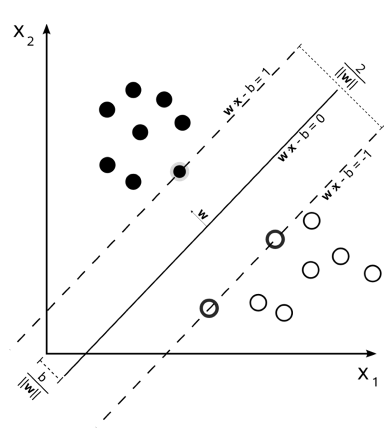
\includegraphics[width=0.6\linewidth]{SVMbilete}}
    \caption{Eit sampel x vert klassifisert til ei klasse basert på om $w^Tx + b>1$ eller $w^Tx + b<1$. Dette gjev to nye grensevektorar som vert kalla støttevektorar
    som høvesvis er gjevne ved $w^Tx + b=1$ og $w^Tx + b=-1$.
    Intuitivt kan ein tenkja på støttevektorane som ein veg. Marginen er lengda på vegen medan avgjerdsgrensa er delelinja på vegen.
    Ein forsøkjer å byggja ein veg som er så brei som mogleg mellom datapunkta, altså så stor margin som mogleg.
    Ut i frå likningane vil ein margin vera på 2 då støttevektorane femner verdiar frå -1 til 1. Ein må samstundes normalisera med lengda til w, så marginen vert
    $\frac{2}{||w||}$.}
    \label{SVMbilete}
\end{figure*}

Eit problem oppstår når ein skal nytta denne teorien for ei ikkje lineært separabel datamengde.
Då finst det inga løysing for optimiseringsproblemet:
\[J(w)=\frac{1}{2}||w||^2 \qquad \text{gjeve føresetnaden $y_i(\frac{g(x_i)}{||w||})\geq \frac{1}{||w||}$}\]
Det vil koma sampel innanføre støttevektorane som impliserer at føresetnaden ikkje er oppfyllt.
Vektorar innanføre støttevektorane som vert klassifisert rette er $0\leq y_i(\frac{w^Tx_i+b}{||w||}) < 1$.
Misklassifiserte vektorar er $y_i(\frac{w^Tx_i+b}{||w||}) < 0$.
Merk at sampel innanføre marginen kan framleis verta klassifisert rette,
men for å få formulert ei løysing vert ein annan variant av SVMar naudsynt då minimiseringskrava ikkje vil vera oppfylte.
Dette kan gjerast ved å introdusera slappare krav for føresetnadane eller at det vert definert løysingar som handsamar ikkje-lineære avgjerdsgrenser.
\subsection{SVM for ikkje-lineært separable datamengder}
Når det ikkje direkte finst ei lineær avgjerdsgrense for problemet finst det fleire variantar av SVM-maskiner som kan koma til nytte.
Ein kan leggja til ein slackparameter $\xi_i$ på den opphavlege optimeringsføresetnaden så $y_i(w^Tx_i+b)=1-\xi_i$.
Dette svarar til å leggja til ein straffeparameter i optimeringsproblemet.
\begin{center}
  Under føresetnaden om at \[y_i(w^Tx_i+b)=1-\xi_i \qquad \xi_i \geq 0 \qquad \forall i\]
  Så vert optimeringsproblemet nå gjeve som å minimisera
\[J(w)=\frac{1}{2}||w||^2+C\sum_{i=1}^N I(\xi_i) \qquad \text{medan $I(\xi_i)=\begin{cases}
       1 &\quad \xi_i>0 \\
       0 &\quad \xi_i=0
     \end{cases}$}\]
\end{center}
%$\xi$ er ein vektor.
Ut frå føresetnaden om at $y_i(w^Tx_i+b)=1-\xi_i$ så vil $\xi_i=0$ femna datapunkta som er korrekt klassifiserte men samstundes er utanføre eller på marginen.
Om $0\leq \xi_i \leq 1$ så er datapunkta riktig klassifiserte samstundes som dei er innanføre marginen. Om $\xi_i=1$ så er datapunkta feilklassifiserte samstundes som dei er innanføre marginen.
Optimiseringsmålet er nå å framleis minimisera marginen, men òg å halda talet på punkt med $\xi_i>0$ så lite som mogleg.
C kontrollerer kor mykje misklassifiserte treningssampel er vekta. Dette problemet kan løysast med lagrangemultiplikatorar som er skildra i ein eigen seksjon.

Dette optimiseringsproblemet har ei meir grafisk tolking.
Søket etter det perfekte hyperplanet som separerer to datamengder er det same som å søkja etter dei to næraste punkta i dei to tilsvarande konvekse mengdene til datamengdene.

Ei konveks mengde kan verta uttrykt som
\[conv\{X\}=\{ y | y=\sum_{i=1}^N \lambda_i x_i \in X, \sum_{i=1}^N \lambda_i=1, 0<\lambda_i<1\}\]
Ein ser her på alle moglege punkt innanføre heile mengda, og ser at ingen av dei er utanføre.
Intuisjonen er lett å sjå om ein berre tenker på randpunkta i mengda. $\sum_{i=1}^N \lambda_i x_i$ er ei vekting av alle
randpunkta som gjev punkt innanføre desse randpunkta, altså punkt i den konvekse mengda. Er $\lambda=1$ ser ein berre på eitt punkt i mengda.
I den reduserte mengda i tydinga nedanføre vert difor ikkje randpunkta med i mengda. Om $\lambda$ er negativ så er
punktet utanføre mengda og vert ikkje med.

Ei redusert konveks mengde er å avgrensa $\lambda_i$ ytterlegare:
\[rconv\{X\}=\{ y | y=\sum_{i=1}^N \lambda_i x_i \in X, \sum_{i=1}^N \lambda_i=1, 0<\lambda_i<\mu\}\]
Der $\mu$ er eit tal mellom 0 og 1. Målet er å gjera så dei to konvekse hulla for kvar av datamengdene ein skal separera
ikkje er overlappande. Det kan ein gjera ved å variera på $\mu$. Når ein har funne dei to konvekse hulla som ikkje overlappar
så vil den beste avgjerdsgrensa vera gjeven som hyperplanet midt mellom dei to næraste punkta i dei to konvekse hulla.

$\mu$ er nært relatert til $C$ i likninga ovanføre. Ein høg C og ein høg $\mu$ vil gjeva nesten overlapp mellom dei konvekse mengdene.

Ei anna løysing for å få ikkje-lineære avgjerdsgrenser med SVMar er med eit kerneltriks skildra i ein eigen seksjon.
Dette vert nytta om mengda definitivt ikkje er lineært separabel.
Om mengda så vidt er lineær separabel kan ei løysing med slack vera meir relevant.
\subsection{Løysing av optimeringsproblem for SVMar}
Alle dei ovannemnde optimeringsproblema for SVM kan løysast med lagrangemultiplikatorar.
Ved å nytta teorien bak lagrangemultiplikatorar får ein følgjande definisjon på dei ovannemnde optimiseringsproblema:
\[{\cal L}(\lambda,b,\boldsymbol{w})=\frac{1}{2}\boldsymbol{w}^T\boldsymbol{w}-\sum_{i=1}^n\lambda_i\left[y_i(\boldsymbol{w}^T\boldsymbol{x}_i+b)-1\right]\]
Problemet må oppfylla Karush–Kuhn–Tucker (KKT) føresetnadane \cite{Sergios}, altså at:
\[\frac{\partial {\cal L}}{\partial b} = -\sum_{i} \lambda_iy_i=0, \qquad \frac{\partial {\cal L}}{\partial \boldsymbol{w}} = 0 = \boldsymbol{w}-\sum_{i} \lambda_iy_i\boldsymbol{x}_i \quad \forall i\]
\[\lambda_i \geq 0 \qquad \lambda_i\left[y_i(\boldsymbol{w}^T\boldsymbol{x}_i+b)-1\right]=0 \]
Under desse føresetnadane vert problemet gjeve som
\[{\cal L}=\sum_i\lambda_i-\frac{1}{2}\sum_{ij}^n\lambda_i\lambda_jy_iy_j\boldsymbol{x}_i^T\boldsymbol{x}_j \qquad \text{Gjeve $\lambda_i\geq 0$ og $\sum_i\lambda_iy_i=0$}\]
Altså skal ein finna maksimum av ${\cal L}$ under desse føresetnadane.
%Under føresetnaden om at $\lambda_i\geq 0$ og $\sum_i\lambda_iy_i=0$.
Ut frå føresetnadane vert det tydeleg at om $\lambda > 0$ så vil $y_i(\boldsymbol{w}^T\boldsymbol{x}_i+b)=1$, altså er punktet $x_i$ på avgjerdsgrensa.
Om $y_i(\boldsymbol{w}^T\boldsymbol{x}_i+b)> 1$ så er $x_i$ ikkje på avgjerdsgrensa så då vert det definert at $\lambda_i=0$.

Ved Karush–Kuhn–Tucker (KKT) føresetnaden $\frac{\partial {\cal L}}{\partial \boldsymbol{w}} = 0$ får ein eit uttrykk for $\boldsymbol{w}$:
\[\boldsymbol{w}=\sum_{i} \lambda_iy_i\boldsymbol{x}_i\]

Og ut i frå $y_i(\boldsymbol{w}^T\boldsymbol{x}_i+b)=1$ kan ein få eit uttrykk for $b$:
\[b = \frac{1}{y_i}-\boldsymbol{w}^T\boldsymbol{x}_i\]

Nå som ein ut frå ein lagrangemultiplikator har fått ei løysing på hyperplankoeffisientane $\boldsymbol{w}$ og $b$ kan ein klassifisera einkvan observasjon $x$ ved:
\[y_i = \mathrm{sign}(\boldsymbol{w}^T\boldsymbol{x}_i+b) \qquad \text{medan $\mathrm{sign}(x) = \begin{cases}
-1 & \text{if } x < 0, \\
0 & \text{if } x = 0, \\
1 & \text{if } x > 0. \end{cases}$}\]
\subsection{Kerneltrikset}
Kerneltrikset er eit triks både for ei raskare løysing av optimiseringsproblemet for SVMar samstundes som det opnar for ikkje-lineære avgjerdsgrenser.
Som vist i ein eigen seksjon om løysing av optimeringsproblem for SVMar så vert løysinga knytt til den følgjande lagrangefunksjonen
\[{\cal L}=\sum_i\lambda_i-\frac{1}{2}\sum_{ij}^n\lambda_i\lambda_jy_iy_j\boldsymbol{x}_i^T\boldsymbol{x}_j\]
Indreproduktet $\boldsymbol{x}_i^T\boldsymbol{x}_j$ kan introdusera særs mange multiplikasjonar. Til dømes om $x$ har dimensjon $(10000x1)$
så vert det ei matrise på $(10 000,10 000)$ som i si utrekning introduserer 100 000 000 multiplikasjonar. Vert det nytta ein særskild kernelfunksjon er det mogleg å
få berre kring 10 000 multiplikasjonar, så kerneltrikset har eit stort potensial til å gjera optimaliseringsproblemet mindre komplekst.
Om ein definerer ein kernelfunksjon $K(\boldsymbol{x}_i,\boldsymbol{x}_j)$ får ein då lagrangefunksjonen på forma:
\[{\cal L}=\sum_i\lambda_i-\frac{1}{2}\sum_{ij}^n\lambda_i\lambda_jy_iy_jK(\boldsymbol{x}_i,\boldsymbol{x}_j)\]
Kernelfunksjonar er i si generelle form gjevne som:
\[K(\boldsymbol{x}_i,\boldsymbol{x}_j)=\phi(\boldsymbol{x}_i)^T\phi(\boldsymbol{x}_j) \]
Der $\phi$ er definert som ei lineæravbilding til eit rom som uttrykker problemet enklare. Korleis avbildinga gjer utrekninga enklare er særs problembunde.
Ofte er målet ved kerneltrikset ikkje berre motivert av raskare utrekningar men òg å få ei ikkje-lineær avgjerdsgrense.
Så lenge kernelfunksjonen utgjer eit indreprodukt for eit og anna indreproduktrom så vert det ikkje naudsynt å nytta avbildinga $\phi$ direkte til rommet.

Ein ønskjer i praksis berre å minimisera med omsyn på eit og anna indreprodukt som gjev ei lineær avgjerdsgrense i det aktuelle indreproduktrommet. Avbildinga vert gjord indirekte med mål om ei lineær avgjerdsgrense i det transformerte rommet, sjå Fig. ~\ref{kerneltrick}.
Ein går altså frå eitt rom med ei ikkje-lineær avgjerdsgrense til eit anna rom med ei
lineær avgjerdsgrense.

\begin{figure*}[h!]
    \centering
    \centerline{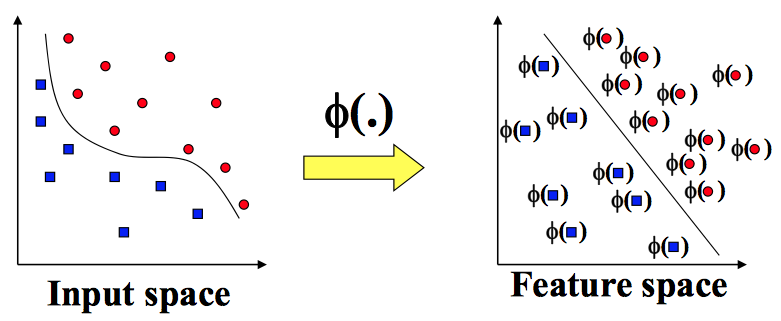
\includegraphics[width=1\linewidth]{kerneltrick}}
    \caption{Avbildinga $\phi$ i ein generell kernelfunksjon vert gjord indirekte i kernelfunksjonen med mål om å transformera datamengda til eit nytt indreproduktrom der avgjerdsgrensa vert lineær.}
    \label{kerneltrick}
\end{figure*}
\newpage
\section{Recurrent Neural Networks (RNN)}
For å klassifisera dei ulike signala med MLPar vart det naudsynt med ei eigenskapsuttrekking då signala åleine ikkje
kunne gjevast til MLPen. I eit tradisjonelt feedforwardnettverk er kvar observasjon prossessert individuelt då det er ingen nettverkstilstand
som held fram under prossesseringa av fleire observasjonar. Det finst der i mot eit anna type nettverk som har tilstand over fleire tidssteg
som opnar opp for at tidlegare prossesserte observasjonar kan ha innverknad på dei neste observasjonane som skal prossesserast.
Dette nettverket vert kalla eit recurrent neural network.

Eit recurrent neural network (vidare nemnt som RNN) er ei utviding av eit nevralt nettverk med ei tilbakekopling i kvart gøymde lag så
kvar nervecellekopling utgjer retta sykliske grafar. Ein RNN kan difor tolkast som ei utviding av eit vanleg feedforwardnettverk så
sykliske nervecellekoplingar vert tillatne. Dette gjer at nettverket har ei form for internt minne av kva som har vorte rekna ut tidlegare.
Det gjer at desse nettverka er særleg gode på sekvensiell data.

For å opna opp for ein RNN skal læra ut frå fleire posisjonar i den sekvensielle datamengda så vert vektmatrisene mellom alle laga delte.
Samstundes er den fundamentale sykliske strukturen til RNN bygd opp sånn at desse nettverka ofte får ein dyp struktur.
Dette leier til det fundamentale problemet med RNN. I eit slikt tilfelle vil backpropagationalgoritmen gjera at særskilde gradientverdiar
anten eksploderer i verdi eller kverv mot 0. Dette problemet er kjent i litteraturen som «the vanishing (and exploding) gradient problem».
Dette gjer at den sekvensielle dybda vert særs avgrensa. I praksis vil eit RNN nettverk berre fungere med 10-20 observasjonar \cite{Goodfellow-et-al-2016}.
Til samanlikning utgjer eit vanleg EEG-signal 4097 observasjonar i datamengda, så det vert naudsynt med ei anna vinkling for å løysa problemet.
% akkurat som i differenslikningar.
% I likskap med differenslikningar så er output òg bunde av tidlegare utrekningar.
\subsection{Long Short-Term Memory RNN (LSTM)}
Det finst ein variant av RNNar kalla Long Short-Term Memory RNN (vidare nemnd som LSTM) som forsøkjer å unngå problema knytte
til oppdatering av gradientverdiane i ein vanleg RNN. Ein LSTM utvider teorien bak RNN med ein algoritme som finkontrollerer
oppdateringa av minnestrukturen i det gøymde laget. Dette vert gjort ved å introdusera tre forskjellige portar som kontrollerer flyten
inn og ut av minnestrukturen.

\begin{figure*}[h!]
    \centering
    \centerline{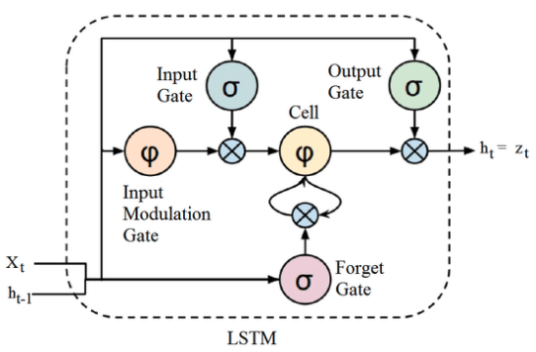
\includegraphics[width=1\linewidth]{LSTMcell}}
    \caption{LSTM si løysing på problema knytte til ein vanleg RNN er å introdusera tre portar som kontrollerer oppdatering av minne; ein inputport, ein «forget»-port og ein outputport. Inputporten og outputporten avgjer høvesvis kva
    som skal vera input og output for minnestrukturen. «forget»-porten avgjer kva som skal gløymast i minnestrukturen. Saman kontrollerer dei at
    ingen gradientar eksploderer i verdi eller kverv mot 0.}
    \label{LSTMcell}
\end{figure*}

\chapter{Resultat}        %% ... or ??
Merk: med mindre det er eksplisitt nemnt noko anna vil alle køyringane i resultatdelen vera gjorde med omsyn på testmengda.
\section{Resultat for eigenskapsuttrekking ved PCA}
Som tidlegare nemnt vart det naudsynt med ei eigenskapsuttrekking frå signala for både MLPar, SVMar og logistiske regresjonsmetodar.
Til det vart dei følgjande eigenskapane nytta: gjennomsnitt, standardavvik, kurtose, skeivskap samt verdiar for min/max.
Desse eigenskapane er nært korrelerte. Det vart difor gjort ein prinsipalkomponentanalyse med omsyn på desse eigenskapane.
Resultatet gav at dei to første prinsipalkomponentane femner kring $0.98$ prosent av den totale variansen. Resten av komponentane skildra særs lite av variansen og vart utelatne.
Så alt i alt reduserte PCA frå 6 eigenskapar ned til 2.
\newpage
\section{Resultat for logistisk regresjon}

\begin{figure*}[h!]
  \begin{subfigure}{\textwidth}
        \centering
        \centerline{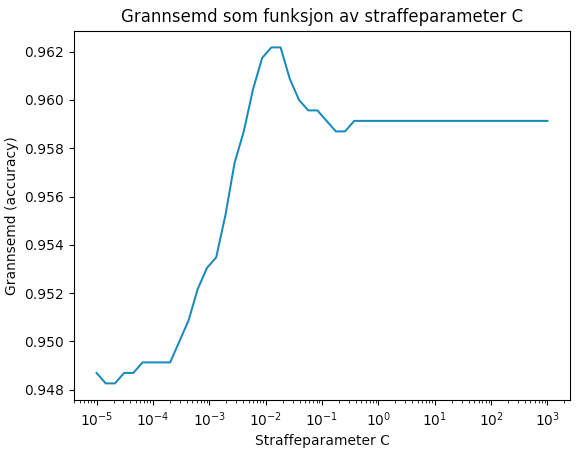
\includegraphics[width=0.7\linewidth]{LR_L2}}
        \caption{Grannsemda for logistisk regresjon som funksjon av straffeparameter C med l2-norm for straffeparameteren. Det beste resultatet vert oppnått kring $10^{-2}$ med kring 0.962 i grannsemd.}
        \label{LRL2}
    \end{subfigure}
\end{figure*}

\begin{figure*}[hb!]
  \begin{subfigure}{\textwidth}
        \centering
        \centerline{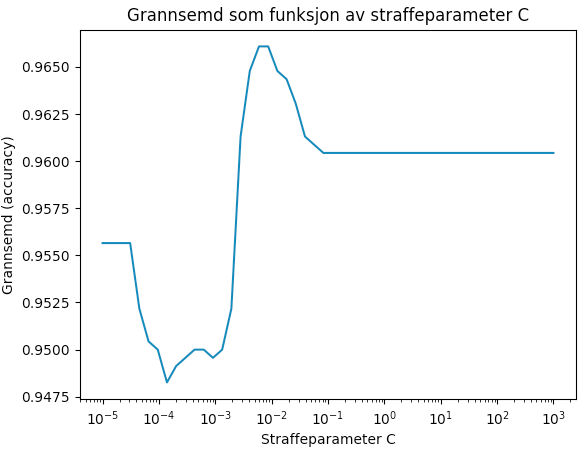
\includegraphics[width=0.7\linewidth]{LR_L1}}
        \caption{Grannsemda for logistisk regresjon som funksjon av straffeparameter C med l1-norm for straffeparameteren. Altså tilsvarande plott som i Fig. ~\ref{LRL2}, berre med omsyn på ein l1-norm for straffeparameteren i staden for l2-norm.
        Ein optimal straffeparameter vert funnen kring $10^{-2}$ med kring 0.965 i grannsemd, altså vil det beste resultatet med omsyn på l1-norm for straffeparameteren vera kring 0.03 betre i grannsemd enn for l2-normen. l1-norm på straffeparameteren vil altså gjeva betre grannsemd enn l2-norm.}
        \label{LRL1}
    \end{subfigure}
\end{figure*}


\begin{figure*}[h!]
  \begin{subfigure}{\textwidth}
        \centering
        \centerline{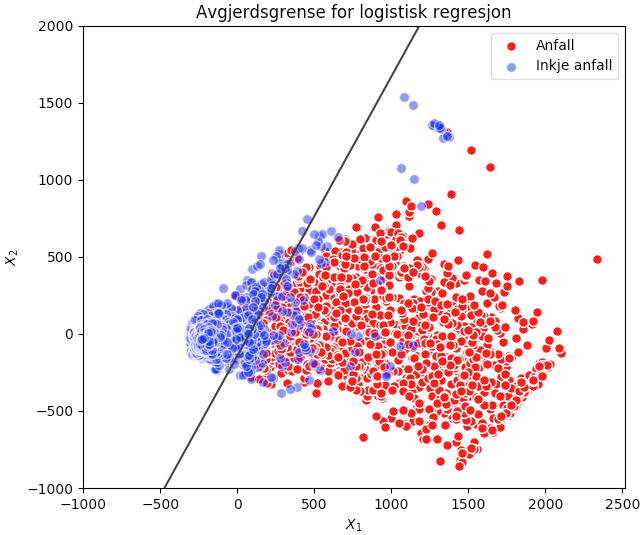
\includegraphics[width=1\linewidth]{LR}}
        \caption{Scatterplot med avgjerdsgrense. Denne lineære avgjerdsgrensa oppnådde den beste grannsemda for logistisk regresjon med 0.9652 i grannsemd. Programmet vart køyrt med l1-norm for straffeparameteren med ein straffeparameter på $5 \cdot 10^{-3}$. Sjølv om plottet viser at fleire punkt overlappar så vert denne avgjerdsgrensa altså ganske god. Dei to eigenskapane $X_1$ og $X_2$ vart resultatet frå PCA. Saman skildrar $X_1$ og $X_2$ 98 prosent av den totale variansen. }
        \label{LRPlot}
    \end{subfigure}
\end{figure*}
\newpage\phantom{blabla}
\section{Resultat for SVM}
Resultat med omsyn på ymse kernelfunksjonar på forma $K(\boldsymbol{x}_i,\boldsymbol{x}_j)=\phi(\boldsymbol{x}_i)^T\phi(\boldsymbol{x}_j)$: \\
\begin{figure*}[h!]
  1. Lineær kernelfunksjon: $K(\boldsymbol{x},\boldsymbol{y})=\boldsymbol{x}^T\boldsymbol{y}$: \\\\
  \begin{subfigure}{\textwidth}
        \centering
        \centerline{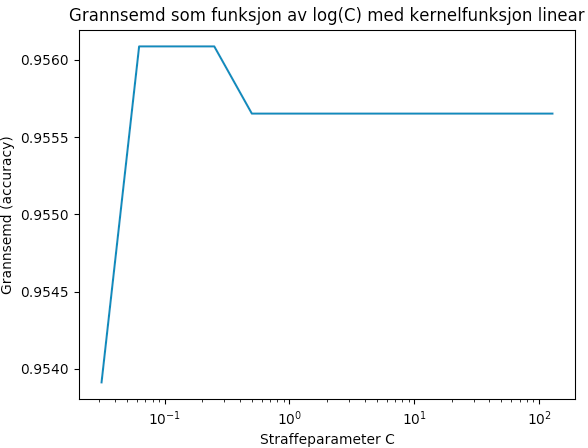
\includegraphics[width=0.8\linewidth]{linear}}
        \caption{Grannsemd som ein funksjon av straffeparametrar C i logaritmisk skala. Her er det ikkje venta noko betre resultat enn for logistisk regresjon då avgjerdsgrensa med denne kernelfunksjonen framleis vil vera lineær. Plottet stadfestar også dette.}
        \label{linear}
    \end{subfigure}
\end{figure*}
\newpage
\begin{figure*}[h!]
  2. Polynomiell kernelfunksjon: $K(\boldsymbol{x},\boldsymbol{y})=(\boldsymbol{x}^T\boldsymbol{y}+\gamma)^d$: \\\\
  \begin{subfigure}{\textwidth}
        \centering
        \centerline{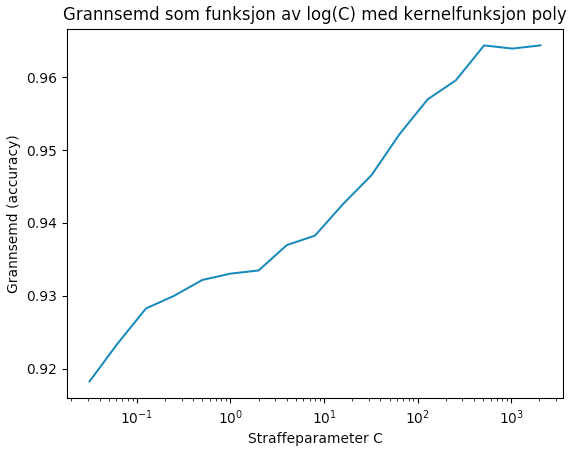
\includegraphics[width=0.7\linewidth]{poly}}
        \caption{Grannsemd som ein funksjon av straffeparametrar C i logaritmisk skala. Plottet vart laga med omsyn på dei parametrane som gav best resultat - ein polynomgrad på 3 samstundes som $coef0=0.01$.
         Grannsemda flatar ut med $0.965$ i verdi kring $10^3$ i straffeparameterverdi.}
        \label{poly}
    \end{subfigure}
\end{figure*}

\begin{figure*}[h!]
  3. Gaussian Radial Basis Function: $K(\boldsymbol{x},\boldsymbol{y})=\exp{\left(-\gamma\vert\vert\boldsymbol{x}-\boldsymbol{y}\vert\vert^2\right)}$: \\\\
  \begin{subfigure}{\textwidth}
        \centering
        \centerline{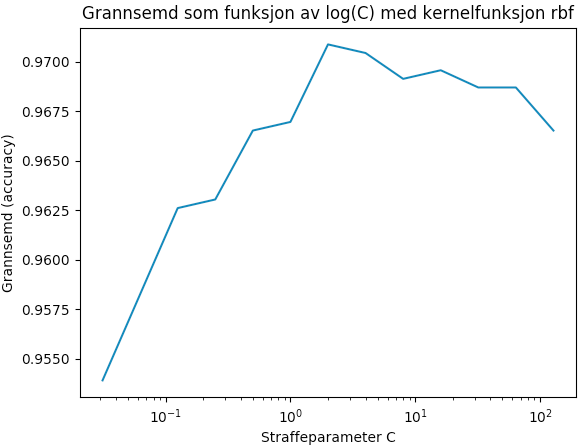
\includegraphics[width=0.7\linewidth]{rbf}}
        \caption{Grannsemd som ein funksjon av straffeparametrar C i logaritmisk skala. Beste oppnådde grannsemd kom på ~0.97. Denne kernelfunksjonen gav altså det beste resultatet for SVMar.}
        \label{rbf}
    \end{subfigure}
\end{figure*}

\begin{figure*}[h!]
  4. Sigmoid kernel: $K(\boldsymbol{x},\boldsymbol{y})=\tanh{(\boldsymbol{x}^T\boldsymbol{y}+\gamma)}$: \\\\
  \begin{subfigure}{\textwidth}
        \centering
        \centerline{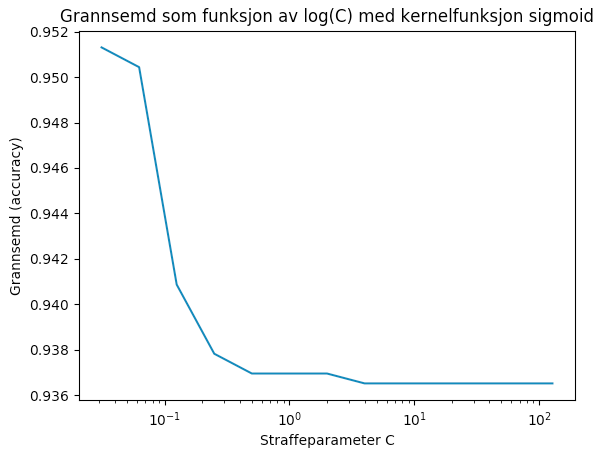
\includegraphics[width=0.8\linewidth]{sigmoid}}
        \caption{Grannsemd som ein funksjon av straffeparametrar C i logaritmisk skala. Denne kernelfunksjonen gjorde det dårlegast, særleg ved høge straffeverdiar.}
        \label{sigmoid}
    \end{subfigure}
\end{figure*}

\section{Resultat for MLPar}

\begin{figure*}[h!]
\begin{center}
  \begin{tabular}{c c c c c | c}
  Læringsrate & Epokar & Batchstorleik & Tal på lag & Nerveceller & Grannsemd \\
  \hline
      0.04 & 136 & 32 & 2 & $[521, 6]$ & 0.971 \\
      0.04 & 143 & 64 & 1 & $[298]$ & 0.968 \\
      0.04 & 191 & 32 & 2 & $[247, 359]$ & 0.963 \\
      0.3 & 178 & 64 & 1 & $[429]$ & 0.952
  \end{tabular}
 \end{center}
 \caption{Dei beste oppnådde resultata med sjølvimplementert nevralt nettverk frå prosjekt 2. Kolonnen «Nerveceller» gjev for kvar køyring ein array med talet på nerveceller for lag l gjeve ved indeks l i arrayen. }
 \label{bestMLPs}
\end{figure*}
Resultata for sci-kit og eiga implementering vart oppnådde ved eit tilfeldig søk gjennom utvalde parameterintervall, sjå vedhenget for resultat knytte til scikit-learn.
Det vart gjort forsøk med å nytta same søkealgoritme med keras si MLP implementering, men det vart ganske treigt i samanlikning.
Så det vart i staden gjort parametersøk med eiga implementering før dei same parametrane vart køyrde med keras si implementering.
\begin{figure*}[h!]
\begin{center}
  \begin{tabular}{c c c c c | c}
  Læringsrate & Epokar & Batchstorleik & Tal på lag & Nerveceller & Grannsemd \\
  \hline
      0.04 & 136 & 32 & 2 & $[521, 6]$ & 0.9583 \\ % 0.9548
      0.04 & 143 & 64 & 1 & $[298]$ & 0.9557 \\ % 0.9509
      0.04 & 191 & 32 & 2 & $[247, 359]$ & 0.9626 \\
      0.3 & 178 & 64 & 1 & $[429]$ & 0.9487
  \end{tabular}
 \end{center}
 \caption{Dei same parametrane som i Fig. ~\ref{bestMLPs} køyrde med keras si implementering av MLPar og Adamoptimizeren. Kolonnen «Nerveceller» gjev for kvar køyring ein array med talet på nerveceller for lag l gjeve ved indeks l i arrayen. }
 \label{bestMLPsKeras}
\end{figure*}

\begin{figure*}[h!]
\begin{center}
  \begin{tabular}{c c c c c | c}
  Læringsrate & Epokar & Batchstorleik & Nerveceller & \% av treningsmengde & Grannsemd \\
  \hline
      0.04 & 136 & 32 & $[521, 6]$ & 100 & 0.971 \\
      0.04 & 136 & 32 & $[521, 6]$ & 10 & 0.956 \\
      0.04 & 136 & 32 & $[521, 6]$ & 5 & 0.950
  \end{tabular}
  \caption{Det beste resultatet for MLPar med omsyn på ymse prosentdelar av den totale treningsmengda. Det er tydeleg at det med MLPar framleis vert særs gode resultat tross i ei redusert treningsmengde. Kolonnen «Nerveceller» gjev for kvar køyring ein array med talet på nerveceller for lag l gjeve ved indeks l i arrayen. }
  \label{bestMLPsYmse}
 \end{center}
\end{figure*}
\newpage\phantom{blabla}
%\newpage\phantom{blabla}
\section{Resultat for LSTMar}
Det største problemet med LSTMar var den lange treningstida. Det beste resultatet med to LSTM-lag hadde ei treningtid på over 100 minutt for ein epoke. Det å gjera ei form for gridsearch eller eit tilfeldig søk i utvalde intervall var difor fåfengt.
Parameterrommet vart i staden undersøkt ved få utvalde køyringar med aktuelle parametrar med ei så avgrensa utrekningstid som mogleg.
\begin{figure*}[h!]
\begin{center}
  \begin{tabular}{c c c c c | c}
  Tid (min) & Epokar & Batchstorleik & Tal på LSTM-lag & Nerveceller & Grannsemd \\
  \hline
      270 & 3 & 4 & 2 & $[128, 64, 2]$ & 0.963 \\
  \end{tabular}
 \end{center}
 \caption{Beste oppnådde resultat for keras sin LSTM. Etter kring 35 minutt vil grannsemda liggja stabilt på minst $0.93$, men vidare går det veldig treigt. Etter over 4 timar låg grannsemda stabilt over 0.96.
 Det siste laget er alltid eit densely-connected lag, medan dei andre er LSTM-lag. Kolonnen «Nerveceller» gjev for kvar køyring ein array med talet på nerveceller for lag l gjeve ved indeks l i arrayen.}
 \label{bestLSTMs}
\end{figure*}

\begin{figure*}[h!]
\begin{center}
  \begin{tabular}{c c c c c | c}
  Tid (min) & Epokar & Batchstorleik & Nerveceller & \% av total treningsdata & Grannsemd \\
  \hline
      270 & 3 & 4 & $[128, 64, 2]$ & 100 & 0.963 \\
      41 & 3 & 4 & $[128, 64, 2]$ & 10 & 0.9535 \\
      20 & 3 & 4 & $[128, 64, 2]$ & 5 & 0.9397
  \end{tabular}
 \end{center}
 \caption{Det beste resultatet for LSTMar med omsyn på ymse prosentdelar av den totale treningsmengda. Samanlikna med tidlegare tabell Fig. \ref{bestMLPsYmse} så vert det tydeleg at både MLPar og LSTMar framleis gjev gode resultat sjølv med ei særs redusert treningsmengde. Kolonnen «Nerveceller» gjev for kvar køyring ein array med talet på nerveceller for lag l gjeve ved indeks l i arrayen. }
 \label{bestLSTMs}
\end{figure*}

\section{Filstruktur for koden}
\begin{itemize}
\item Det meste av datahandsaminga vert gjort i «LastData.py».
\item All koden knytt til SVMar vert funnen i «SVMTestar.py».
\item All koden knytt til RNN/LSTM vert funnen i «NevraltNettRNN.py».
\item All koden knytt til logistisk regresjon vert funnen i «LogistiskRegresjonTestar.py».
\item All koden knytt til testar av MLP med eiga implementering ligg i «NevraltNettEigenMLP.py»
\item All koden knytt til testar av MLP med Keras ligg i «NevraltNettKerasMLP.py»
\end{itemize}
\chapter{Perspektiv og konklusjonar}                     %% ... or Konklusjon
Frå resultata er det tydeleg at MLPar, LSTMar og SVMar gav dei beste resultata. Det er så lite som skil dei ulike metodane i grannsemd at det vert særs vanskeleg å konkludera objektivt med
kva for ein metode som gjer det best. Som vist kan MLPar gjeva gode resultat om det vert gjort ei god eigenskapsuttrekking på førehand. Det beste oppnådde resultatet for MLPar var 0.97.

LSTMar krev inga eigenskapsuttrekking av signala men med kompromisset om at trening er særs tidkrevjande.
Dette har gjort at det er lite sannsynleg at dei optimale parametrane for klassifiseringsproblemet er funne for LSTMar. Det beste oppnådde resultatet for LSTM vart 0.963.
Alle metodane fungerer også særs godt ved reduserte treningsmengder. For berre 5 prosent av den originale treningsmengda held LSTMar og MLPar seg framleis over $0.95$ i grannsemd.

SVMar fekk resultat kring $0.97$ i likskap med MLPar om det vart nytta anten gaussian radial basis kernel eller ein polynomiell kernelfunksjon.
Sigmoid og ein lineær kernelfunksjon gav framleis gode resultat på kring 0.95 på sitt beste. Logistisk regresjon med si lineære avgjerdsgrense fekk $0.965$ som beste grannsemd.
Med berre eitt sekund med måledata vil alle metodane i rapporten gjeva særs gode resultat. Alle metodane skildra i rapporten får minst 0.95 i grannsemd.

Framtidig arbeid knytte til klassifisering av EEG-signal ved MLPar, SVMar og logistiske regresjonsmetodar vil i stor grad vera retta mot ei undersøking av betre eigenskapar.
Det har vore fleire lovande publikasjonar som undersøkjer eigenskapar knytte til den diskrete wavelettransformen av EEG-signal, til dømes publikasjonen frå
Manisha Chandani og Arun Kumar i American Journal of Information Science and Technology \cite{DWT}.
Resultata deira ved ei eigenskapsuttrekking med diskret wavelettransform for SVMar og MLPar kom kring $0.99-1$ i grannsemd,
samanlikna med eiga implementering som fekk 0.97 som beste resultat. Det er også mykje rom for å undersøkja parameterromma betre.
\newpage
Som tidlegare nemnt var eit stort problem med LSTM nettverk at dei tek særs lang tid å trena og at parameterromma difor har vorte dårleg undersøkte.
Eit eventuelt framtidig arbeid vil for LSTM heilt klart vera å undersøkja parameterrommet betre.
Det finst samstundes òg fleire variantar av RNN som kan vera betre enn LSTM, ein annan variant av RNN kalla Gated Recurrent Unit (GRU) er
venta å gjeva ei kortare treningstid enn LSTM for dette problemet. GRU er særs lik LSTM men har betre treningstid på kortare signal.
\chapter{Vedheng}                     %% ... or ?? # 0p01,10p0,100p0
\begin{figure*}[h!]
\begin{center}
  \begin{tabular}{c c c c c | c}
  Læringsrate & Epokar & Batchstorleik & Tal på lag & Nerveceller & Grannsemd \\
  \hline
      0.04 & 136 & 32 & 2 & $[521, 6]$ & 0.9665 \\
      0.04 & 143 & 64 & 1 & $[298]$ & 0.9643 \\
      0.04 & 191 & 32 & 2 & $[247, 359]$ & 0.9526 \\
      0.3 & 178 & 64 & 1 & $[429]$ & 0.9486
  \end{tabular}
 \end{center}
 \caption{Utvalde køyringar med scikit-learn si MLP implementering. Det vart nytta dei same parametrane som i Fig. ~\ref{bestMLPs} og Fig. ~\ref{bestMLPsKeras}. Kolonnen «Nerveceller» gjev for kvar køyring ein array med talet på nerveceller for lag l gjeve ved indeks l i arrayen. }
 \label{bestMLPsSkikit}
\end{figure*}
\backmatter{}
\printbibliography
\end{document}
